\documentclass[tikz,border=10pt]{standalone}

% Prior approaches organized by query model: each oracle hits its own barrier.
% Bottom banner: this work (additive queries) breaks the exponential barrier.

\usepackage{tikz}
\usetikzlibrary{arrows.meta,calc,positioning}
\usepackage{amsmath,amssymb}
\usepackage{xcolor}

\definecolor{barrierc}{RGB}{200,50,50}
\definecolor{priorc}{RGB}{110,110,110}
\definecolor{oursc}{RGB}{0,140,60}
\definecolor{oraclec}{RGB}{0,100,200}

\begin{document}
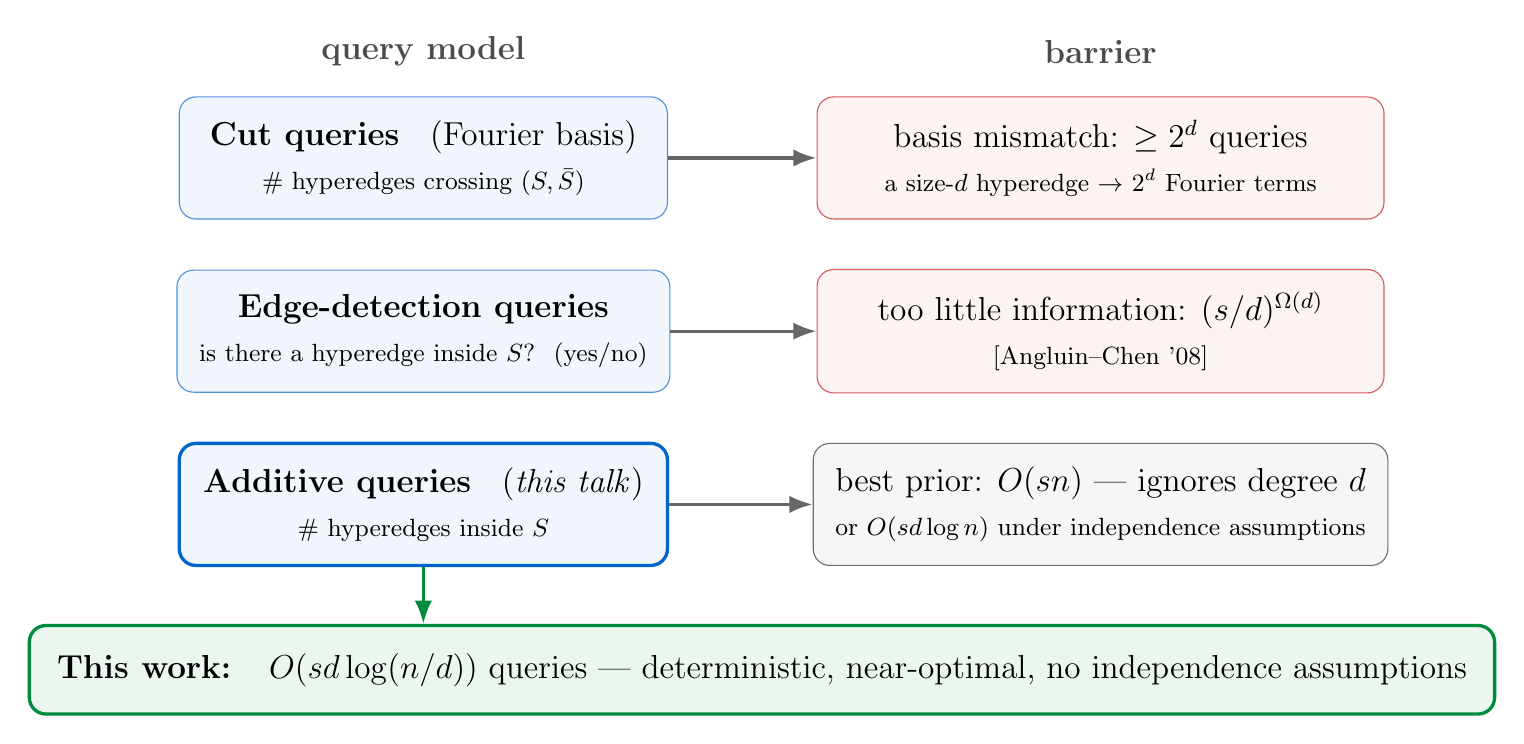
\begin{tikzpicture}[
  oracle/.style={draw=oraclec!70, fill=oraclec!6, rounded corners=6pt, align=center,
                 inner sep=8pt, minimum width=6.2cm, minimum height=1.55cm, font=\large},
  barrier/.style={draw=barrierc!80, fill=barrierc!6, rounded corners=6pt, align=center,
                  inner sep=8pt, minimum width=7.2cm, minimum height=1.55cm, font=\large},
  prior/.style={draw=priorc, fill=priorc!6, rounded corners=6pt, align=center,
                inner sep=8pt, minimum width=7.2cm, minimum height=1.55cm, font=\large},
  ours/.style={draw=oursc, fill=oursc!8, rounded corners=6pt, align=center,
               inner sep=10pt, line width=1.2pt, font=\large},
  imp/.style={-Latex, very thick, black!60},
]

% column headers
\node[font=\large\bfseries, black!70] at (0, 1.35) {query model};
\node[font=\large\bfseries, black!70] at (8.6, 1.35) {barrier};

% Row 1: cut queries
\node[oracle] (o1) at (0,0)
  {\textbf{Cut queries} \; (Fourier basis)\\[2pt] \small \# hyperedges crossing $(S, \bar S)$};
\node[barrier] (b1) at (8.6,0)
  {basis mismatch: $\geq 2^{d}$ queries\\[2pt] \small a size-$d$ hyperedge $\to$ $2^d$ Fourier terms};
\draw[imp] (o1.east) -- (b1.west);

% Row 2: edge-detection queries
\node[oracle] (o2) at (0,-2.2)
  {\textbf{Edge-detection queries}\\[2pt] \small is there a hyperedge inside $S$? \;(yes/no)};
\node[barrier] (b2) at (8.6,-2.2)
  {too little information: $(s/d)^{\Omega(d)}$\\[2pt] \small [Angluin--Chen '08]};
\draw[imp] (o2.east) -- (b2.west);

% Row 3: additive queries (our setting)
\node[oracle, draw=oraclec, line width=1.2pt] (o3) at (0,-4.4)
  {\textbf{Additive queries} \; (\emph{this talk})\\[2pt] \small \# hyperedges inside $S$};
\node[prior] (b3) at (8.6,-4.4)
  {best prior: $O(sn)$ --- ignores degree $d$\\[2pt] \small or $O(sd\log n)$ under independence assumptions};
\draw[imp] (o3.east) -- (b3.west);

% Ours banner
\node[ours] (banner) at (4.3,-6.5)
  {\textbf{This work:} \; $O(sd \log(n/d))$ queries --- deterministic, near-optimal, no independence assumptions};
\draw[imp, oursc] (o3.south) -- (o3.south |- banner.north);

\end{tikzpicture}
\end{document}
